\begin{figure*}
  \centering
  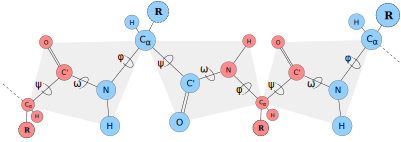
\includegraphics[width=0.75\textwidth]{figures/protein-torsion-angles}
  \caption{Illustration of the protein torsion angles in a protein
    subsequence of three amino acids.}
  \label{fig:protein-torsion-angles}
\end{figure*}

The representation of proteins shown in the structure diagram of
Figure \ref{fig:amino_connect} is suitable for determining the
chemical properties of the molecules, getting an overview of how atoms
are arranged and how the atoms are connected. However, to get an exact
model of the protein structure we need a lot more precision in our
characterization. That is, we need to include the concepts of bond
lengths, bond angles and torsional angles into the model.  Figure
\ref{fig:protein-torsion-angles} illustrates the concepts.

\subsection{Data set}
In the next sections we have used a collection of proteins from
Protein Data Bank\footnote{\url{http://www.pdb.org}} to obtain suitable
values for the bond lengths and bond angles of proteins. We have
downloaded a set of 645 protein descriptions (randomly chosen from the
site). We have verified the values we present in Table
\ref{tab:average_bond_lengths} and Table \ref{tab:average_bond_angles}
by comparing them to those obtained by \cite{probik} and
\cite{laskowski1993main}.

\section{Backbone geometry}
\textit{Bond lengths} are the distances between the covalently bonded atoms
in a molecule (usually measured in ångstrøm). We will name the
individual bond lengths by the name of the two atoms which the bond
connects. For example, the bond between a \Ca\ and N atom in an amino acid of
the protein backbone is called \Ca -N. We have computed bond lengths
for all bonds in the backbone, the results are shown in Table
\ref{tab:average_bond_lengths}. As can be seen from the last column in
the table, the variation is very limited and we therefore have not
found it necessary to consider any variations from the mean
lengths. 
%% Actually, these variations are so small that they can very possibly
%% be attributed to uncertainty in the measuring equipment.

\begin{table}
  \centering
  \begin{tabular}{lrr}
    \toprule
    \multicolumn{1}{c}{Bond} & \multicolumn{1}{c}{Avg. length} & \multicolumn{1}{c}{Std.dev.} \\ \midrule 
    C-O   & 1.2260 Å & 0.0188 Å\\
    CA-C  & 1.5272 Å & 0.0191 Å\\
    N-CA  & 1.4680 Å & 0.0237 Å\\
    C-N   & 1.3234 Å & 0.0215 Å\\
    N-H   & 0.9793 Å & 0.0342 Å\\
    CA-CB & 1.5327 Å & 0.0228 Å\\
    CA-HA & 1.0747 Å & 0.0307 Å\\ \bottomrule
  \end{tabular}
  \vspace{1mm}
  \caption{Average bond lengths (in ångstrøm)}
  \label{tab:average_bond_lengths}
\end{table}

A \textit{bond angle} is an angle between two outgoing bonds from a
single atom. As an example, the angle between the bonds N-\Ca\ and \Ca
-C' is called N-\Ca -C'. Table \ref{tab:average_bond_angles} shows
average values for the backbone bond angles in degrees. Again can we
see that the variation is very limited, but as a small angular
displacement can have a rather large influence on the remaining part
of the protein, they could still introduce variability into the model
of much larger order. In this project we have however chosen to
focus solely on the variability in the torsional angles, thus locking
the bond angles to their mean values.

\begin{table}
  \centering
  \begin{tabular}{l>{$}r<{^\circ$}>{$}r<{^\circ$}}
    \toprule
    \multicolumn{1}{c}{Bond} & \multicolumn{1}{c}{Avg. angle} & \multicolumn{1}{c}{Std.dev.} \\ \midrule 
    H-N-CA & 118.9553 & 1.9979\\
    N-CA-C & 110.6099 & 2.4668\\
    CA-C-O & 120.7088 & 1.3064\\
    CA-C-N & 116.7804 & 1.7682\\
    C-N-CA & 121.4547 & 1.9946\\
    C-N-H  & 119.5112 & 2.1599\\ \bottomrule
  \end{tabular}
  \vspace{1mm}
  \caption{Average bond angles (in degrees)}
  \label{tab:average_bond_angles}
\end{table}

A \textit{torsional angle} is a rotational angle around a bond. In the
backbone, there are three such torsional angles (see Figure
\ref{fig:protein-torsion-angles}). The $\phi$ and $\psi$ angles were
mentioned earlier and we will return to them after this paragraph. The
last one, the $\omega$-angle, is almost always $180^{\circ}$
\cite{probik}, but at a few occurrences it deviates from this
value. We will assume that the $\omega$ angle is \textit{always}
$180^{\circ}$. This makes the grey rectangular areas of Figure
\ref{fig:protein-torsion-angles} completely rigid.  Each of the
torsional angles can be defined as dihedral angles between two
planes. For example, the $\phi$ angle can be described by the angle
between the two planes defined by the atoms C$_{n-1}'$, N$_n$ and \Ca
$_n$ as well as N$_n$, \Ca $_n$ and C$_n'$. Thus, four atoms are
needed to define a dihedral angle.

Getting back to the $\phi$ and $\psi$, we can now see that these are
the main variability of the protein backbone, as all bond lengths and
bond angles are nearly rigid and the $\omega$-angle rarely
deviates from $180^\circ$. 

Because of collisions between the backbone and the side-chains (and in part also the backbone itself), some combinations of $\phi$ and $\psi$ angles are more probable than others. The probability of the angle combinations can be illustrated graphically in what is known as a
\textit{Ramachandran plot} (Figure \ref{fig:ramachandran}). In the
plot on the left a Ramachandran probability map for all
amino acids except glycine are shown. And in the right plot a probability map
values for glycine are shown. Glycine is special because of its
simplicity. It consists of a single H atom connected to the $C_\alpha$
of the amino acid and thus collisions with the backbone is hardly ever
a problem.

\begin{figure*}
	\centering
	\subbottom[]{\hspace{0.5cm}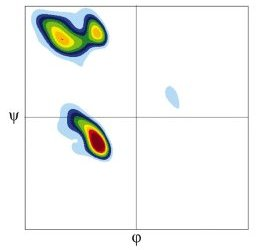
\includegraphics[width=0.3\textwidth]{figures/ramachandran_except_gly}\hspace{0.5cm}}
    \subbottom[]{\hspace{0.5cm}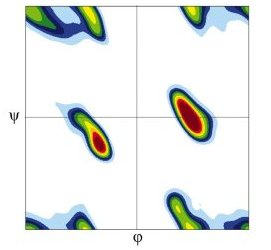
\includegraphics[width=0.3\textwidth]{figures/ramachandran_only_gly}\hspace{0.5cm} \label{fig:ramachandran_gly}}
    \caption{\textbf{(a)} A Ramachandran plot for all amino
      acids except Glycine. \textbf{(b)}  Ramachandran plot
      for Glycine. The illustration is taken from Wikipedia.}
\label{fig:ramachandran}
\end{figure*}
%\fxwarning{Evt. tilføj  $-180^\circ$, $0^\circ$ og $180^\circ$ på akserne i Ramachandran plots}

% \subsection{Additional measurements}
% To place the atoms we have had the need to obtain further measures

\section{Side-chain geometry}
\begin{figure}
	\centering
	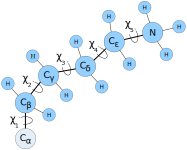
\includegraphics[width=0.42\textwidth]{figures/lysine}
    \caption{Illustration of the torsional $\chi$-angles on the side-chain of Lysine (LYS).}
    \label{fig:lysine-and-chi}
\end{figure}

As for the backbone, the side-chains can be described by bond lengths,
bond angles and a few torsional angles.  The torsional angles of
protein side-chains are named $\chi_1-\chi_5$, but most side-chains
only have the first angle or two. In Figure \ref{fig:lysine-and-chi},
we have illustrated the five $\chi$-angles on the side-chain of the
Lysine amino acid. As can be seen, the first $\chi$ angle defines the
rotation around the $C_\alpha-C_\beta$ bond, and so forth along the
side-chain. Side-chains tend to have certain configurations of their
$\chi$-angles, as we will explain in Section
\ref{chap:handling_sidechains}, such configurations are called
\textit{rotamers}.

To simplify how we construct the proteins, we have chosen to use
another representation than directly measuring all bond lengths and
bond angles as we did for the backbone. For each type of amino acid we
store its side-chain in a coordinate system that has \Ca\ as origin and
orientated such that the first bond, $C_\alpha-C_\beta$, is following
the x-axis. For the calculation of these positions, we have again used
our protein data set and taken the mean position of all atoms when all
torsional angles are set to zero.

Thus, to place a side-chain on a certain \Ca\ of the backbone, we
insert the side-chain atoms, using the offset positions to \Ca\ with
the appropriate rotation using the bond angles to $C_\beta$.

%%% Local Variables: 
%%% mode: latex
%%% TeX-master: "rapport"
%%% End: 
